\section{$PSF$ approximation for fast and distributed deconvolution} \label{gradients}
This section describes our main hypothesis of this work: We can further approximate the $PSF$ in the Major/Minor cycle and exploit it to speed up/distribute coordinate descent based deconvolution algorithms. A deconvolution algorithm receives the residual image from the Major cycle and the $PSF$. Over several iterations, it deconvolves the residual image with the $PSF$, and creates the deconvolved 'model' image of the observation.

A deconvolution algorithm in the Major/Minor cycle works with a $PSF$, which is constant over the whole image. However, this is not the case for modern radio interferometers. The $w$-term in the visibility measurements modify the true $PSF$ over the image. This is why we need the Major cycle: After a number of iterations of the deconvolution algorithm, the Major cycle transforms the model image back to visibility measurements, and subtracts the model from the measured visibilities. Then, it transforms the residual visibilities back into image space. The gridder corrects for the $w$-term. It corrects the error the deconvolution algorithm introduces with a constant $PSF$. The Major cycle allows us to use an approximation of the true $PSF$ in the deconvolution. We believe this can be exploited to speed up/distribute the deconvolution.

\begin{figure}[h]
	\centering
	\begin{subfigure}[b]{0.45\linewidth}
		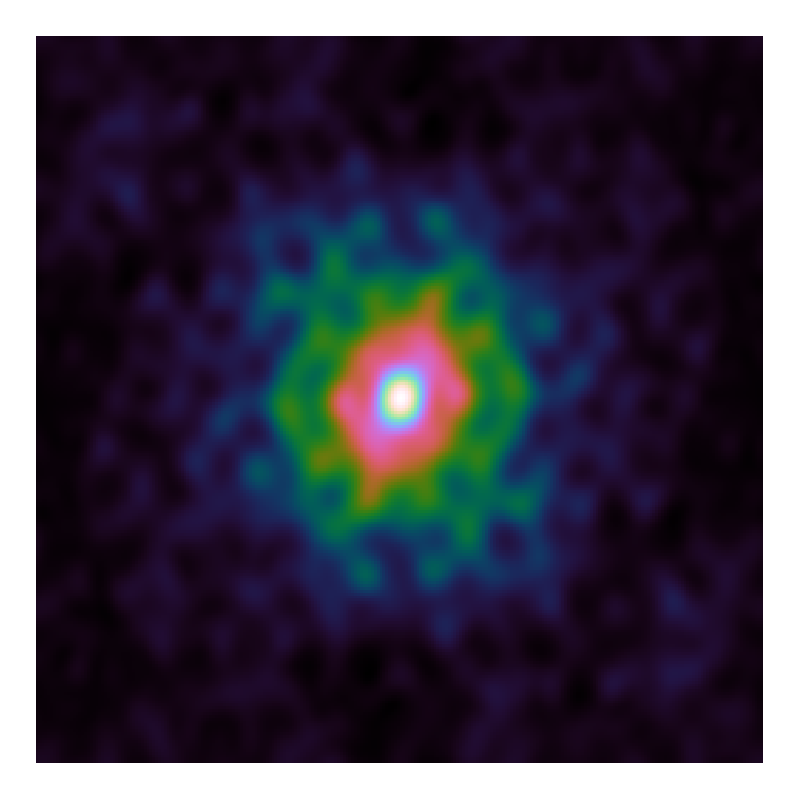
\includegraphics[width=\linewidth, clip, trim= 0.25in 0.25in 0.25in 0.25in]{./chapters/03.cd/simulated/psf.png}
		\caption{Full $PSF$}
	\end{subfigure}
	\begin{subfigure}[b]{0.45\linewidth}
		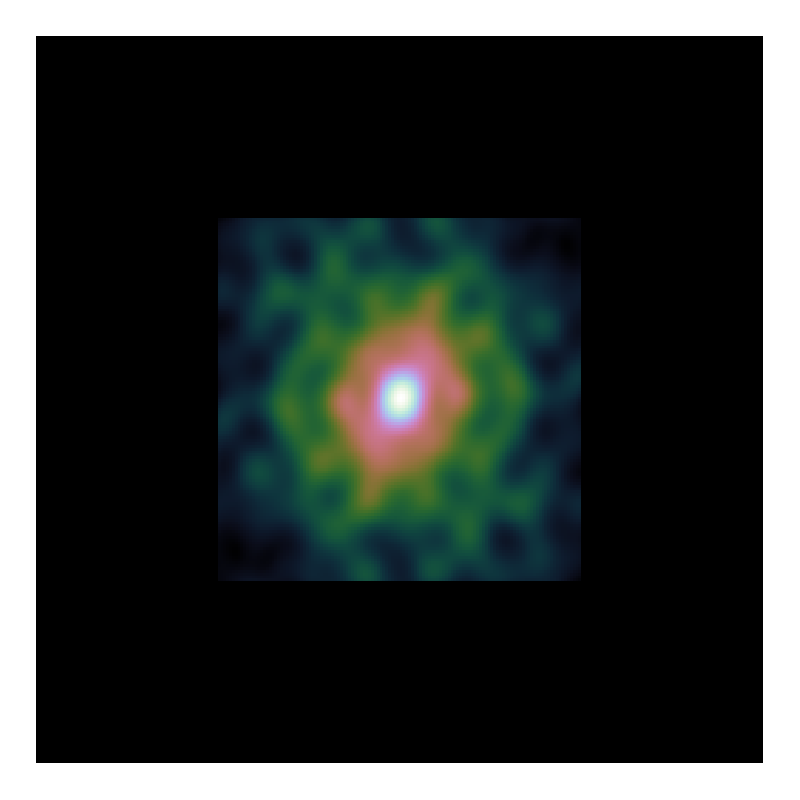
\includegraphics[width=\linewidth, clip, trim= 0.25in 0.25in 0.25in 0.25in]{./chapters/03.cd/simulated/psfCut.png}
		\caption{$\frac{1}{2}PSF$ approximation}
	\end{subfigure}
	\caption{$PSF$ approximation typically used in Clark CLEAN}
	\label{gradients:clark}
\end{figure}

An approximation of the full $PSF$ has already been developed for CLEAN: The Clark CLEAN algorithm \cite{clark1980efficient} uses only a window of the full $PSF$ for the deconvolution. Figure \ref{gradients:clark} shows the full $PSF$ and the approximate $PSF$ used typically in Clark CLEAN. During deconvolution, it only uses a window around the center of the full $PSF$. Typically, the sides of the window is $\frac{1}{2}$ of the image size. By using only a $\frac{1}{2} PSF$ window around the center, a Clark CLEAN iteration is significantly faster than standard CLEAN. With $\frac{1}{2} PSF$, Clark CLEAN has to subtract only the $\frac{1}{2} PSF$ window from the residuals, which is 4 times smaller than the full $PSF$.

Using only a fraction fo the true $PSF$ speeds up the deconvolution. But it also introduces sparsity in the deconvolution problem which, to our knowledge, has not been explored for radio interferometers. The full $PSF$ shown in Figure \ref{gradients:clark} has significant values around the center, but they quickly approach zero the further away we move from the center. If we only use a window around the center $\frac{1}{2} PSF$ and set the rest to zero, we are using a sparse $PSF$. For a CLEAN algorithm, the sparse approximated $PSF$ ignores the influence of far away pixel.

\subsection{$PSF$ approximation and approximate gradient calculation}
Our coordinate descent algorithm minimizes a single pixel in each iteration. It selects a pixel to minimize, calculates its gradient, and descends the towards the gradient direction. In our coordinate descent deconvolution algorithm, the $PSF$ is central to the gradient calculation: The gradient for each pixel can be calculated by correlating the residual image with the $PSF$. 
Calculation of gradients.

Approximate gradients

T

The serial coordinate descent algorithm keeps the gradient map, the product $PSF \star PSF$ and the current reconstruction in memory. In each iteration, the algorithm first finds the pixel, which has the maximum possible difference in this iteration. In the second step, it subtracts the product $PSF \star PSF$ at the correct location of the gradient map. The gradient map is now updated for the next iteration of the serial coordinate descent algorithm.

We approximate the $PSF$ by only using a window around the center. Each side is only a fraction of the full $PSF$ size. From now on, we use the method $Cut()$, which cuts out the center window of the $PSF$. If we use a cut fraction of $\frac{1}{4}$, we cut out a window of the $PSF$, each side being  $\frac{1}{4}$ the length of the full $PSF$.

Using an approximate $PSF$ influences three parts of the serial coordinate descent algorithm: The gradient map, the Lipschitz map and the product $PSF \star PSF$. At the beginning of the algorithm, we calculate the gradient map by correlating the dirty image with the $PSF$ ($I_{dirty} \star PSF$) We also calculate the Lipschitz constants for each pixel. The product $PSF \star PSF$ is used to update the gradient map in each iteration. We developed two approximation methods for the serial coordinate descent algorithm. Method 1 is called 'approximate update', and method 2 is called 'approximate deconvolution'.

T


\subsection{Major Cycle convergence and implicit path regularization}\label{gradients:pathreg}
There is one problem with the approximate $PSF$ which is left to solve: When does the serial coordinate descent algorithm decide to use a Major cycle. Or when we combine the $PSF$ approximation methods, how many Major cycles do we use for each method?

When we use an approximate $PSF$, the deconvolution algorithm will at a certain iteration start to include 'side lobes' of the $PSF$. The Figure \ref{gradient:convergence:sidelobe} shows an example of the side lobes we introduce by approximating the $PSF$ with $\frac{1}{2}$ of the center window. At a certain point, the deconvolution with an approximate $PSF$ has to decide whether the emission is real, or whether it is an artifact from the $PSF$ approximation, and will be removed with the next major cycle.

%re-introduce residuals

\begin{figure}[h]
	\centering
	\begin{subfigure}[b]{0.3\linewidth}
		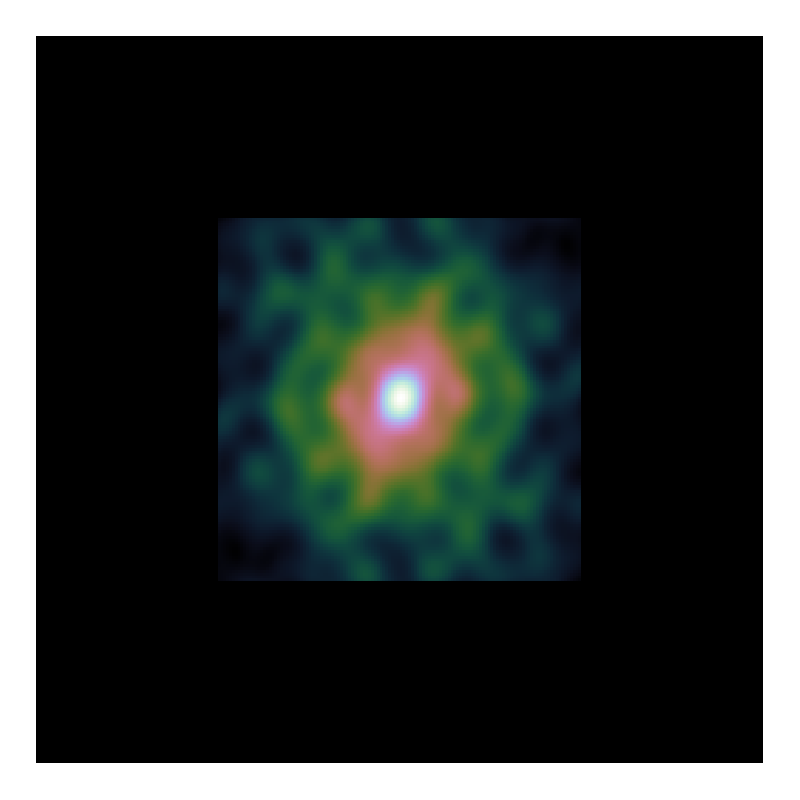
\includegraphics[width=\linewidth, clip, trim= 0.25in 0.25in 0.25in 0.25in]{./chapters/03.cd/simulated/psfCut.png}
		\caption{$\frac{1}{2}PSF$ approximation}
	\end{subfigure}
	\begin{subfigure}[b]{0.3\linewidth}
		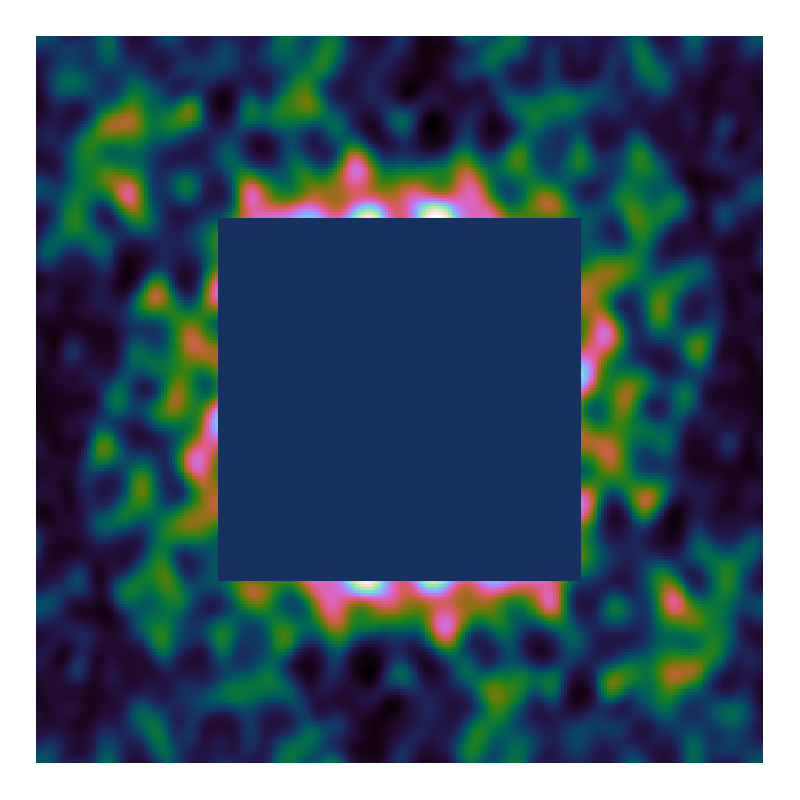
\includegraphics[width=\linewidth, clip, trim= 0.25in 0.25in 0.25in 0.25in]{./chapters/03.cd/simulated/psfReverseCut.png}
		\caption{$PSF$ Sidelobes}
		\label{gradient:convergence:reverseCut}
	\end{subfigure}
	
	\caption{Maximum sidelobe of the $PSF$ cutoff.}
	\label{gradient:convergence:sidelobe}
\end{figure}

For example: if we have an observation with a single point source in the center, the first iteration of Clark CLEAN will subtract the approximate $PSF$ from the residuals. But the residual image is left with the $PSF$ side lobes shown in Figure \ref{gradient:convergence:reverseCut}. The next iteration may detect 'fake' point sources at the significant side lobes of the $PSF$. Our serial coordinate descent algorithm does not explicitly use the residual image, but has a similar problem. The information of the residual image is implicitly contained in the gradient map. Our serial coordinate descent algorithm with an approximate $PSF$ leaves significant gradients in the map.

This is a problem for deconvolving an image with the Major cycle. If we let our serial coordinate descent algorithm converge to a result in each Major cycle, it will include emission from the $PSF$ side lobes. In the next Major cycle, the serial coordinate descent algorithm has to remove the side lobes from the reconstruction, but this again leaves significant side lobes in the gradient map. This can lead to an oscillation of the algorithm, where it adds and removes the same side lobes several times over different Major cycles. In extreme cases (for example when we use an aggressive approximation of the $PSF$), this may even lead to a diverging behavior. But even if the deconvolution algorithm converges over several Major cycles, if the algorithm spends too much time on $PSF$ side lobes, it may become significantly slower.

To solve this problem, we use the following strategy for our serial coordinate descent algorithm: We estimate the $PSF$ side lobes introduced by the approximation. We increase the regularization parameter $\lambda$, until the elastic net regularization excludes all side lobes from the reconstruction. Note that real emission may also be regularized away in the current Major cycle iteration. The serial coordinate descent algorithm reconstructs the image with the current $\lambda$, and lets the Major cycle remove the side lobes. It then estimates the current $PSF$ side lobes for this Major cycle, sets a lower regularization parameter $\lambda$ and again deconvolves the image.

This is known as a path regularization in optimization. We let our optimization algorithm converge on intermediate solution, decrease the $\lambda$ parameter and use the intermediate solution as a 'warm start'. Coordinate descent methods may benefit from path regularization\cite{friedman2010regularization}. Converging on all intermediate solutions may result in a lower wall-clock time than converging directly on the final solution.

We use the path regularization to stop the algorithm from wasting computing resources on side lobes. There may be different strategies that result in an overall lower wall-clock time for the serial coordinate descent algorithm, but they were not explored in this project. We set the regularization parameter $\lambda$ for each Major cycle according to the following estimate:

\begin{equation}
\begin{split}
maxSidelobe &= Max(PSF - Cut(PSF)) \\
gradients &= residuals \star PSF \\
\lambda_{cycle} &= \frac{Max(gradients) * maxSidelobe}{\alpha}\\
\lambda_{cycle} &= Max(\lambda, \lambda_{cycle})
\end{split}
\end{equation}

We calculate the maximum side lobe of the $PSF$ approximation. We then multiply the maximum side lobe with the maximum gradient. This is an estimate of the largest gradient value, which gets left in the gradient map by the $PSF$ approximation. We then set the $\lambda_{cycle}$ parameter to exclude all gradients equal or smaller that gradient magnitude. The maximum of the gradient map decreases over every Major cycle, which leads to a decreasing $\lambda_{cycle}$ until we reached the target value $\lambda$.

This estimate works, but it has one problem for radio interferometric imaging: It does not account for extended emissions. Since they have non-zero pixel values close to each other, their $PSF$ side lobes also overlap. Meaning the $PSF$ side lobes of extended emissions are higher than we estimated. This is why we added a correction factor which estimates how much the maximum in the gradient map is point-source-like:

\begin{equation}
\begin{split}
maxLobe &= Max(PSF - cut(PSF)) \\
gradients &= residuals \star PSF \\
\textbf{corr} &= Max \left [1, \frac{Max(gradients)}{Max(residuals) * Lipschitz} \right ] \\
\lambda_{cycle} &= \frac{Max(gradients) * maxLobe * corr}{\alpha}\\
\lambda_{cycle} &= Max(\lambda, \lambda_{cycle})
\end{split}
\end{equation}

It the same estimate as before, except for the correction factor. The correction factor is 1 if the maximum in the gradient map is a point source, and $1 <$ if the maximum in the gradient map is more like an extended emission. The correction factor is based on the following observation: If the image only contains point sources, then the maximum of the gradient map should be equal the maximum of the residuals times the Lipschitz constant. But if it is an extended emission, the maximum of the gradient map will be significantly larger.

This is the estimate we use for the regularization parameter $\lambda_{cycle}$ for each Major cycle. The parameter $\lambda_{cycle}$ decreases over each Major cycle, resulting in an implicit path regularization for our serial coordinate descent method.
